\documentclass[../2.tex]{subfiles}
\begin{document}
    {\Huge Unstable}\\
    In \autoref{ch:1} we studied homology and cohomology on abstract simplicial complexes, in this chapter we shall discuss in detail
    $1$-dimensional abstract simplicial complexes.

    \begin{defn}
        A \ii{graph} is a $1$-dimensional abstract simplicial complex.
    \end{defn}

    In a graph $\mc{G}$ the non trivial chain groups are therefore $C_0(\mc{G})$ and $C_1(\mc{G})$, also called vertex and edge spaces. 
    The canonical basis of the vertex space is the set of vertexes $\{\ket{i}\}_{i \in I}$, and that of edges which is a subset of $\{\ket{i,j}\}_{(i,j)\in I\times I}$.

    \begin{defn}
        Let $\mc{G}$ be a graph, we define the \ii{adjacency matrix} $A$ of $\mc{G}$ on the canical vertex basis by
        \[a_{ij} = 
        \begin{cases}
            1 & \ket{i,j} \in C_1 \\
            0 & otherwise \\
        \end{cases} \]        
    \end{defn}
    Only one boundary $\del_1$ and one coboundary $\del_1^\dagger$ can be defined on graphs, we shall name their dual representatives  respectively gradient $d_1^\dagger$ and divergence $d_1$.

    \begin{defn}
        Let $\mc{G}$ be a graph, we define the \ii{boundary} $\del_1 : C_1 \to C_0$ by 
        \[ \del_1\ket{i,j} := \ket{i} - \ket{j} \quad \forall \ket{i,j} \in C_1.\]
    \end{defn}
    
    \begin{defn}
        Let $\mc{G}$ be a graph, we define the \ii{coboundary} $\del^\dagger_1 : C_0 \to C_1$ by 
        \[ \del^\dagger_1\ket{i} := \sum_{\ket{i,j} \in C_1} \ket{i,j}.\]
    \end{defn}

    % {\color{red} Disegno che mostra il cobordo di un nodo}

    % The prevously defined generalizd Stokes' theorem is on graphs a discrete version of the divergence theorem.

    % \begin{thm}
    %     Let $\mc{G}$ be a graph, let $\ket{\phi} \in C_0, \ket{\psi} \in C_1$ then $\bra{\phi}\del_1\ket{\psi} = \bra{\psi}\del_1^\dagger\ket{\phi} = (d_1\bra{\phi})\ket{\psi}$.
    % \end{thm}

    % Therefore the integral of the cochain $\ket{\psi}$ over the boundary of $\ket{\phi}$ equals the integral of the divergence of $\ket{\psi}$ over $\ket{\phi}$.

    % {\color{red} Disegno che mostra il teorema della divergenza discreto}

    On a graph that admits non trivial gradient and divergence, we can define a non trivial laplacian operator as the gradient of the divergence.
    Although this might sound strange, the inversion of gradient and divergence in the definition of laplacian is due to the fact that we are representing
    the functions on the graph (cochains) by their dual chains.

    \begin{defn}
        Let $\mc{G}$ be a graph, we define the \ii{$0$-laplacian} $\Delta_0 : C_0 \to C_0$ by 
        \[ \Delta_0 := \del_1 \del^\dagger_1.\]
    \end{defn}

    One intersting propertiy of the $1$-laplacian is that the dimension of its kernel equals the connected components of the graph.
    To illustrate some of the properties of graphs we will refer to the graph in \autoref{fig:2:3}.

    \begin{figure}[H]
        \begin{minipage}{.5\textwidth}
            \centering
            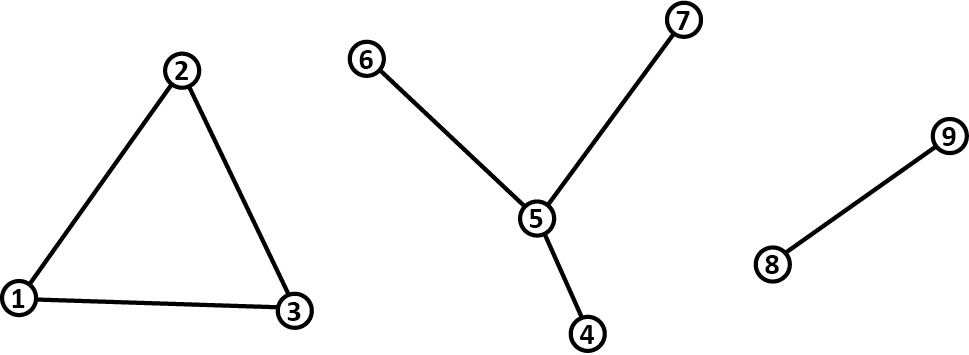
\includegraphics[width=9cm]{sections/2/graphex}
            \caption{The graph.}
            \label{fig:2:3}
        \end{minipage}
        \begin{minipage}{.5\textwidth}
            \centering
            \[\begin{pmatrix}
                0 & 1 & 1 & 0 & 0 & 0 & 0 & 0 & 0 \\
                1 & 0 & 1 & 0 & 0 & 0 & 0 & 0 & 0 \\
                1 & 1 & 0 & 0 & 0 & 0 & 0 & 0 & 0 \\
                0 & 0 & 0 & 0 & 1 & 0 & 0 & 0 & 0 \\
                0 & 0 & 0 & 1 & 0 & 1 & 1 & 0 & 0 \\
                0 & 0 & 0 & 0 & 1 & 0 & 0 & 0 & 0 \\
                0 & 0 & 0 & 0 & 1 & 0 & 0 & 0 & 0 \\
                0 & 0 & 0 & 0 & 0 & 0 & 0 & 0 & 1 \\
                0 & 0 & 0 & 0 & 0 & 0 & 0 & 1 & 0
            \end{pmatrix}. \]
            \caption{Adjacency matrix of the graph.}
            \label{fig:2:4}
        \end{minipage}
    \end{figure}

    \begin{exa}
        Let $\mc{G}$ be the graph  in \autoref{fig:2:3}, then the $0$-laplacian expressed in terms of the canoncal vertex basis $\{\ket{i}\}_{i \in I}$ is

        \[\begin{pmatrix}
                2 & -1 & -1 & 0 & 0 & 0 & 0 & 0 & 0 \\
                -1 & 2 & -1 & 0 & 0 & 0 & 0 & 0 & 0 \\
                -1 & -1 & 2 & 0 & 0 & 0 & 0 & 0 & 0 \\
                0 & 0 & 0 & 1 & -1 & 0 & 0 & 0 & 0 \\
                0 & 0 & 0 & -1 & 3 & -1 & -1 & 0 & 0 \\
                0 & 0 & 0 & 0 & -1 & 1 & 0 & 0 & 0 \\
                0 & 0 & 0 & 0 & -1 & 0 & 1 & 0 & 0 \\
                0 & 0 & 0 & 0 & 0 & 0 & 0 & 1 & -1 \\
                0 & 0 & 0 & 0 & 0 & 0 & 0 & -1 & 1 
            \end{pmatrix}. \] 

        The laplacian matrix is calculated as follows
        \[ \Delta_0 \ket{1} = \del_1\ket{1,2} + \del_1\ket{1,3} = 2\ket{1}-\ket{2}-\ket{3},\]
        \[ \Delta_0 \ket{2} = \del_1\ket{2,1} + \del_1\ket{2,3} = -\ket{1}+2\ket{2}-\ket{3},\]
        \[ \Delta_0 \ket{3} = \del_1\ket{3,1} + \del_1\ket{3,2} = -\ket{1}+-\ket{2}+2\ket{3},\]
        \[ \Delta_0 \ket{4} = \del_1\ket{4,5} = \ket{4}-\ket{5},\]
        \[ \Delta_0 \ket{5} = \del_1\ket{5,4}+\del_1\ket{5,6}+\del_1\ket{5,7} = -\ket{4}+3\ket{5}-\ket{6}-\ket{7},\]
        \[ \Delta_0 \ket{6} = \del_1\ket{6,5} = -\ket{5}+\ket{6},\]
        \[ \Delta_0 \ket{7} = \del_1\ket{7,5} = -\ket{5}+\ket{7},\]
        \[ \Delta_0 \ket{8} = \del_1\ket{8,9} = \ket{8}-\ket{9},\]
        \[ \Delta_0 \ket{9} = \del_1\ket{9,8} = -\ket{8}+\ket{9}.\] 

        Three invariant subspaces emerge from the laplacian, that determine three different laplacians, namely
        \[ \Delta_0 = \Delta_0^\mc{A} \oplus \Delta_0^\mc{B} \oplus \Delta_0^\mc{C}. \]

        Furthermore any of those three blocks has a $1$-dimensional kernel, in fact the dimensional equiations for the laplacians are

        \[dim(ker\Delta_0^\mc{A}) =dimC_0(\mc{A}) - rank
        \begin{pmatrix}
            2 & -1 & -1  \\
            -1 & 2 & -1  \\
            -1 & -1 & 2 
        \end{pmatrix} = 3 - rank
        \begin{pmatrix}
            2 & 0 & -1  \\
            0 & 1 & -1  \\
            0 & 0 & 0 
        \end{pmatrix} = 3 - 2 =  1, \]

        \[ dim(ker\Delta_0^\mc{B}) =dimC_0(\mc{B}) - rank
        \begin{pmatrix}
            1 & -1 & 0 & 0  \\
            -1 & 3 & -1 & -1 \\
            0 & -1 & 1 & 0  \\
            0 & -1 & 0 & 1 
        \end{pmatrix} = 4 - rank
        \begin{pmatrix}
            1 & -1 & 0 & 0  \\
            0 & 2 & 0 & -1 \\
            0 & 0 & 1 & -1  \\
            0 & 0 & 0 & 0 
        \end{pmatrix} = 4 - 3 = 1,\]
        
        \[ dim(ker\Delta_0^\mc{C}) =dimC_0(\mc{C}) - rank
        \begin{pmatrix}
            1 & -1 \\
            -1 & 1
        \end{pmatrix} = 2 - rank
        \begin{pmatrix}
            1 & -1 \\
            0 & 0
        \end{pmatrix} = 2-1 = 1.\]
    \end{exa}

    We can also define an higher dimensional laplacian on the graph.

    \begin{defn}
        Let $\mc{G}$ be a graph, we define the \ii{$1$-laplacian} $\Delta_1 : C_1 \to C_1$ by 
        \[ \Delta_1 := \del_1^\dagger \del_1.\]
    \end{defn}

    One intersting propertiy of the $1$-laplacian is that the dimension of its kernel equals the number of independent cycles.

    \begin{exa}
        In fact we can expand $\Delta_1^\mc{A} := \del_1^\dagger\del_1$ the basis $\{\ket{1,2},\ket{2,3},\ket{3,1}\}$ as
        \[\begin{pmatrix}
            2 & -1 & -1  \\
            -1 & 2 & -1  \\
            -1& -1 & 2 
        \end{pmatrix}.\] 
        The laplacian matrix is calculated as follows
        \[\Delta_1^\mc{A}\ket{1,2} = \del_1^\dagger(\ket{1}-\ket{2}) = 2\ket{1,2}-\ket{3,1}-\ket{2,3},\]
        \[\Delta_1^\mc{A}\ket{2,3} = \del_1^\dagger(\ket{2}-\ket{3}) = -\ket{1,2}+2\ket{2,3}-\ket{3,1},\]
        \[\Delta_1^\mc{A}\ket{3,1} = \del_1^\dagger(\ket{3}-\ket{1}) = -\ket{1,2}+2\ket{3,1}-\ket{2,3}.\]

        We can notice that $\Delta_2$ has a $1$-dimensional kernel.

        \[ dim(ker\Delta_1^\mc{A}) = dimC_1(\mc{A}) - rank
            \begin{pmatrix}
                2 & -1 & 1  \\
                -1 & 2 & 1  \\
                1& 1 & 2 
            \end{pmatrix} = 3 - rank
            \begin{pmatrix}
                2 & 0 & -1  \\
                0 & 1 & -1  \\
                0 & 0 & 0 
            \end{pmatrix} = 3 - 2 =  1. \]

        Since the sum of the three raws is $0$ we can say that the only linearly independent $1$-cycle is $\ket{1,2}+\ket{2,3}+\ket{3,1}$.
    \end{exa}
\end{document}